In alto a destra sulla toolbar è presente un \textbf{menu a tendina}, che permette all'utente due operazioni:
\begin{enumerate}[noitemsep,nolistsep]
    \item Effettuare il \textbf{logout};
    \item Accedere alle \textbf{impostazioni} (solo per utenti di livello \emph{Admin}).
\end{enumerate}
\begin{figure}[H]
    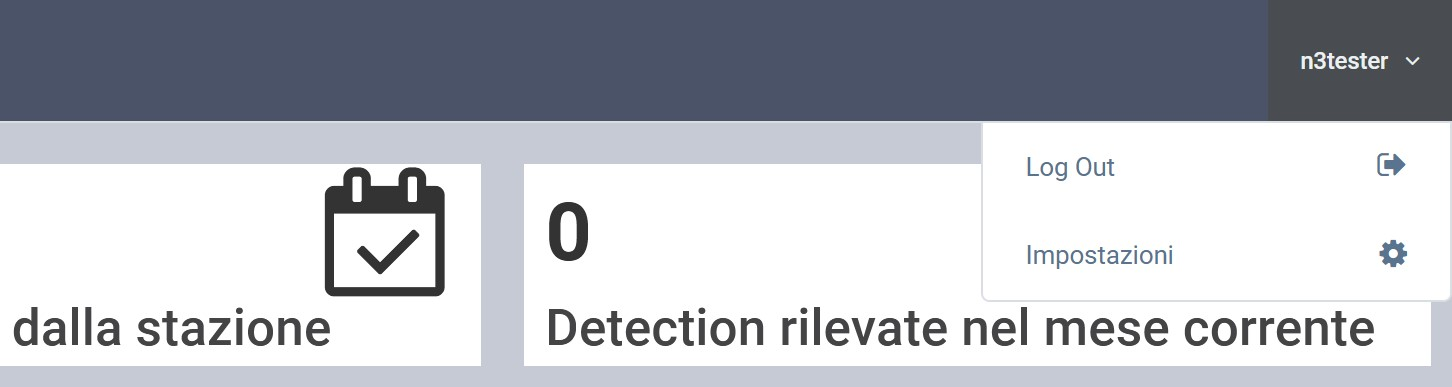
\includegraphics[width=\textwidth]{images/drop-down-menu.jpg}
    \caption{Menu a tendina per utenti di livello \emph{Admin}.}
\end{figure}
Nella pagina delle impostazioni (cfr. figura \ref{fig:settings}) sono presenti due sottosezioni principali:
\begin{itemize}[noitemsep,nolistsep]
    \item \emph{Visualizzazione Media}, per abilitare o disabilitare la visualizzazione delle anteprime o la creazione di video e archivi;
    \item \emph{Archiviazione Media}, per gestire lo spazio sul nodo.
\end{itemize}

\subsection{Disabilitazione visualizzazione anteprime}

Gli amministratori possono decidere, disattivando il \emph{toggle button} corrispondente, di non permettere a qualunque utente acceda alla web application del nodo in questione di visualizzare le anteprime delle sezioni \emph{Capture}, \emph{Stack} e \emph{Detection}, nel caso non si voglia appesantire il nodo con ulteriori elaborazioni ad esempio durante la notte.

\begin{figure}[H]
    
\includegraphics[width=\textwidth]{images/no-preview-toggle.jpg}
\end{figure}

\begin{figure}[H]
    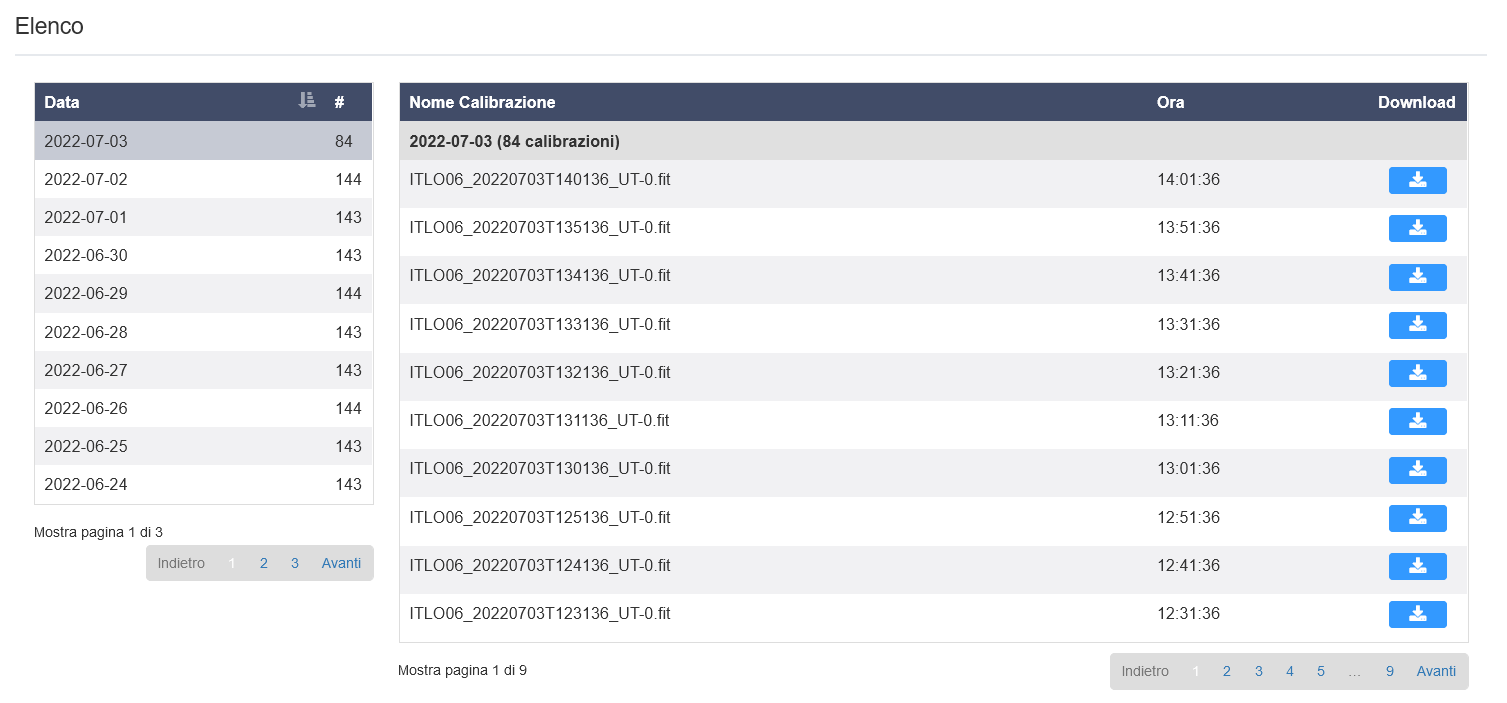
\includegraphics[width=\textwidth]{images/capture-no-preview.png}
    \caption{Sezione \emph{Capture} senza le anteprime. Si noti che non è più presente\emph{toggle button} per attivarle.}
\end{figure}

\subsection{Disabilitazione creazione video e archivio}

Disattivando invece il \emph{toggle button} riguardante i video e gli archivi, gli amministratori possono impedire a qualunque utente che acceda di richiedere lo scaricamento di video o di zip nella sezione \emph{Detection}. Il fine di questa scelta concerne sempre l'utilizzo della risorse sul nodo, soprattutto per non interferire con le elaborazioni del software FreeTure.

\begin{figure}[H]
    
\includegraphics[width=\textwidth]{images/no-download-toggle.jpg}
\end{figure}

\begin{figure}[H]
    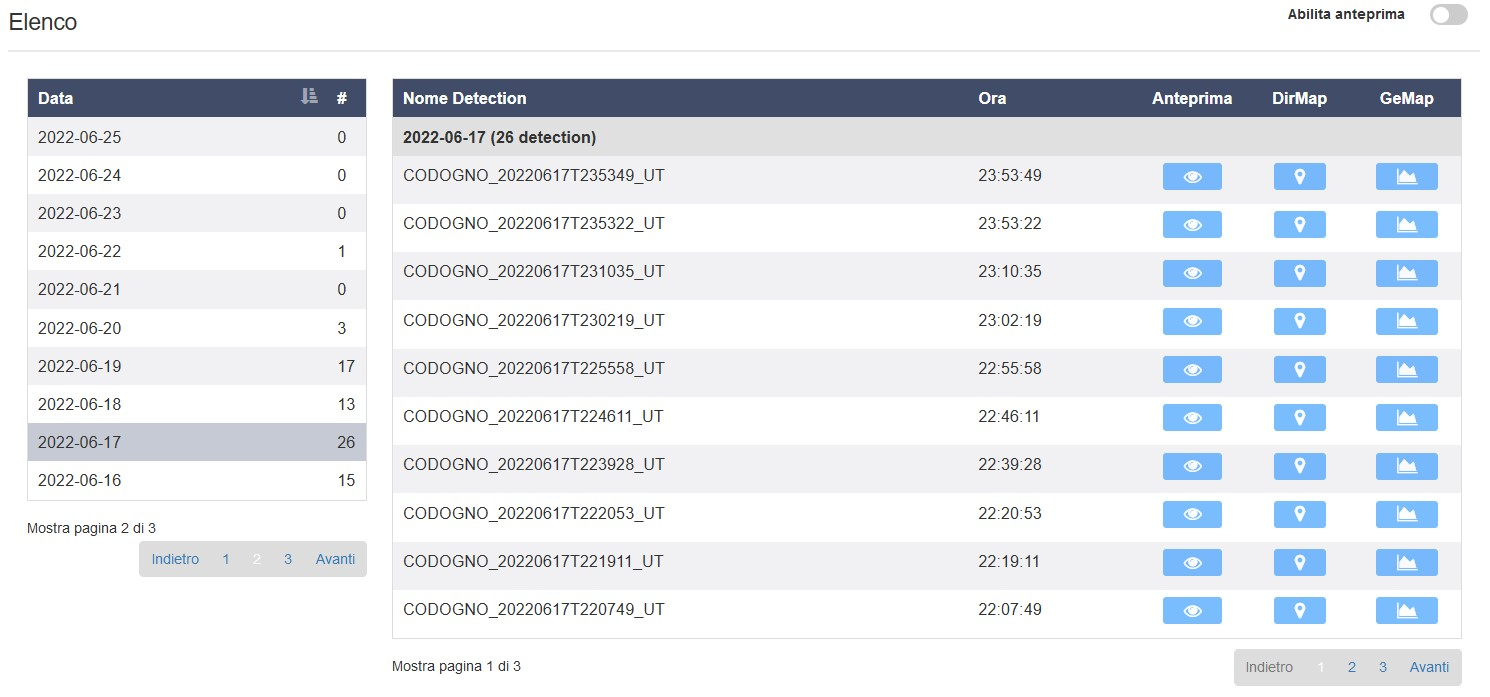
\includegraphics[width=\textwidth]{images/detection-no-download.jpg}
    \caption{Sezione \emph{Detection} senza possibilità di scaricare i video o gli archivi.}
\end{figure}

\subsection{Pulizia media provvisori} \label{clean-media}

\begin{wrapfigure}{r}{0.3\textwidth}
    \vspace{-10pt}
    
\includegraphics[width=0.3\textwidth]{images/clean-media-button.jpg}
    \vspace{-24pt}
\end{wrapfigure}
Nella sezione \ref{elaborazione-dati-detec} si era accennato al fatto che la gestione dei media provvisori sul disco era responsabilità dell'utente.
Nelle impostazioni un amministratore può \textbf{visualizzare quanto spazio occupano in memoria} i video e gli archivi creati precedentemente e quindi decidere se \textbf{liberare lo spazio}, cancellando i media.  

\begin{figure}[H]
    \begin{center}
    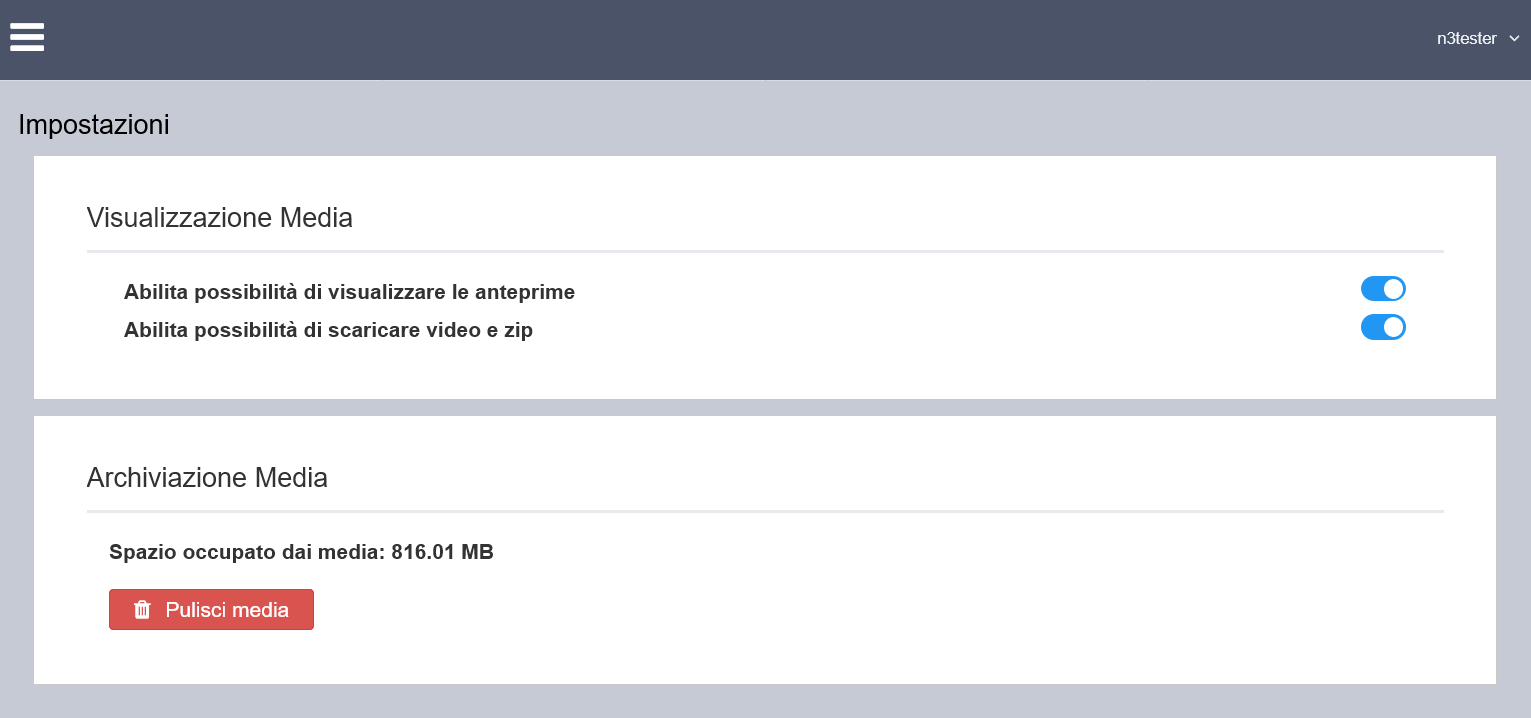
\includegraphics[width=\textwidth]{images/full-settings.png}
    \caption{\emph{Impostazioni}.}
    \label{fig:settings}
    \end{center}
\end{figure}